\section{Computational Rationality}

\textbf{Why User Models}

\textit{Limitations to MHP} \smallskip

\textit{Complexities of real-world tasks} \smallskip


\begin{center}
	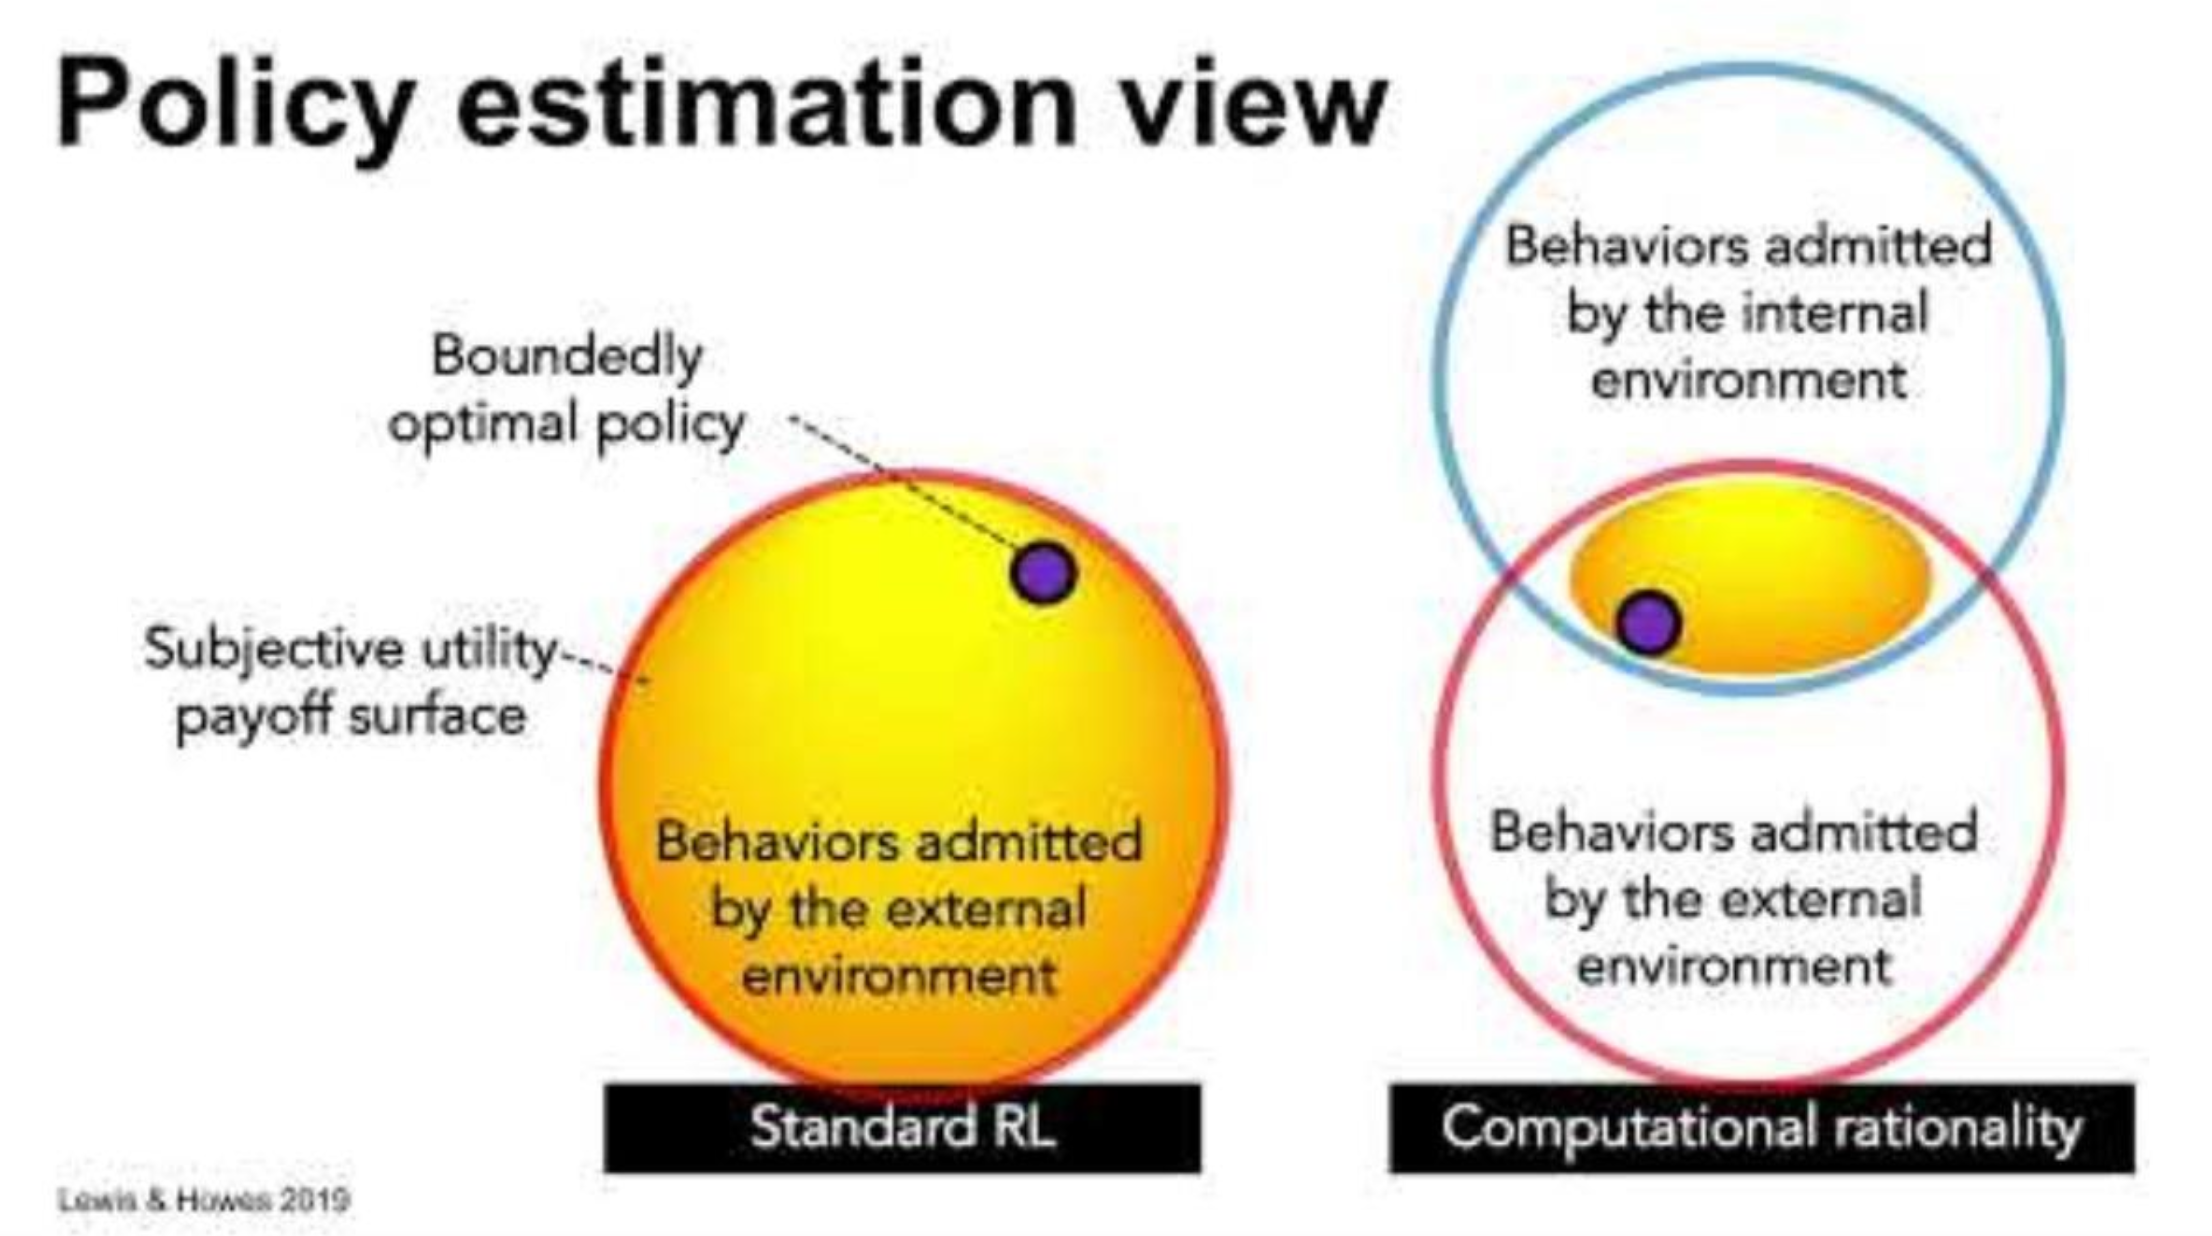
\includegraphics[width=\linewidth]{policy_estimation_view.png}
\end{center}


\textbf{Interactiona s a sequential decision-making process}

\textbf{Optimal Policy}


\textit{Reinforcement Learning} \smallskip


\textit{Difference to other ML paradigms} \smallskip


\textit{Markov Decision Process} \smallskip




\textit{Optimal action given a state} \smallskip


\textit{Value Function} \smallskip

\textit{On Rewards} \smallskip




\textbf{Bounded Rationality}


\textit{Comparison with Standard RL} \smallskip

\textit{Internal vs External Environmen} \smallskip

\begin{center}
	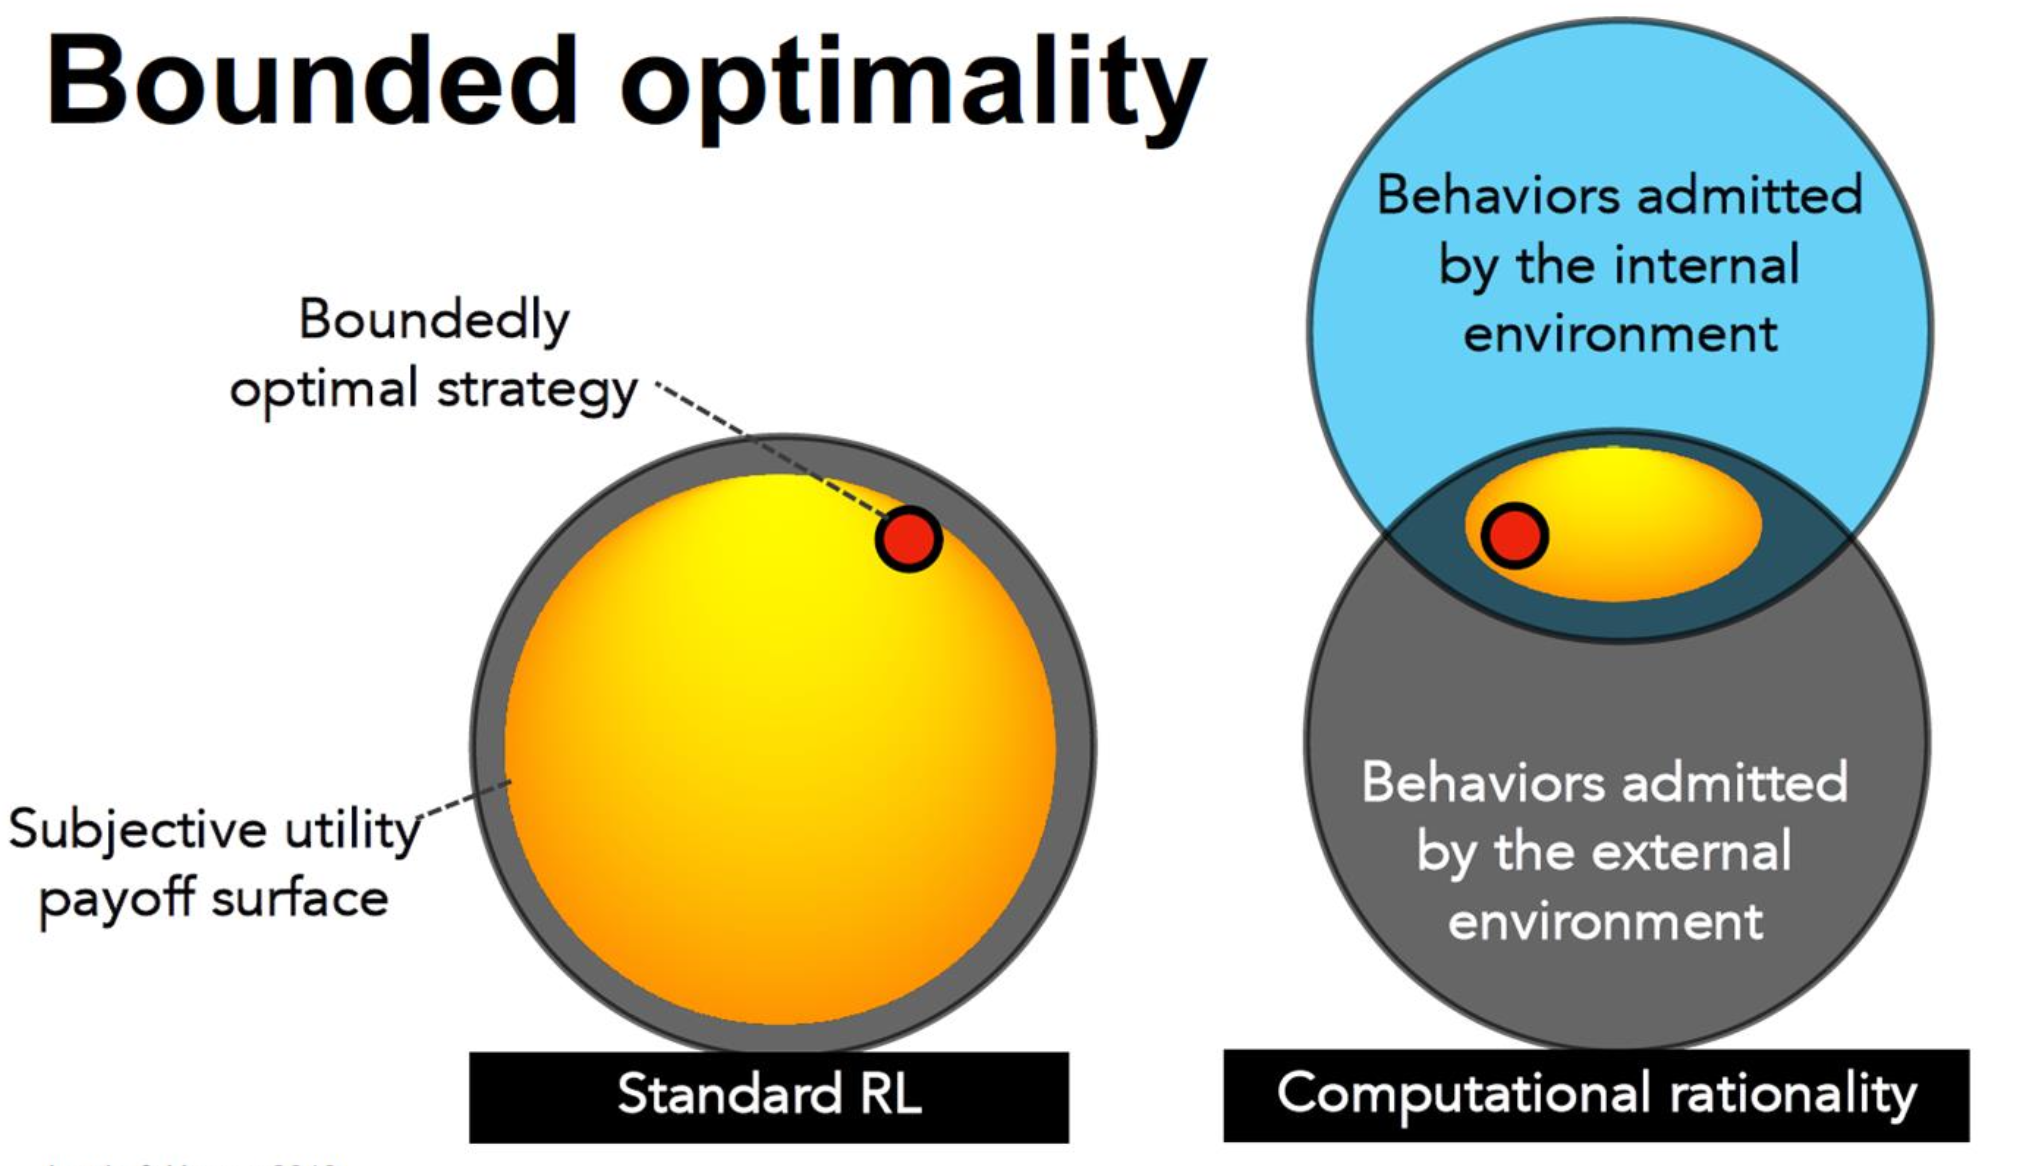
\includegraphics[width=\linewidth]{bounded_optimality.png}
\end{center}


\begin{center}
	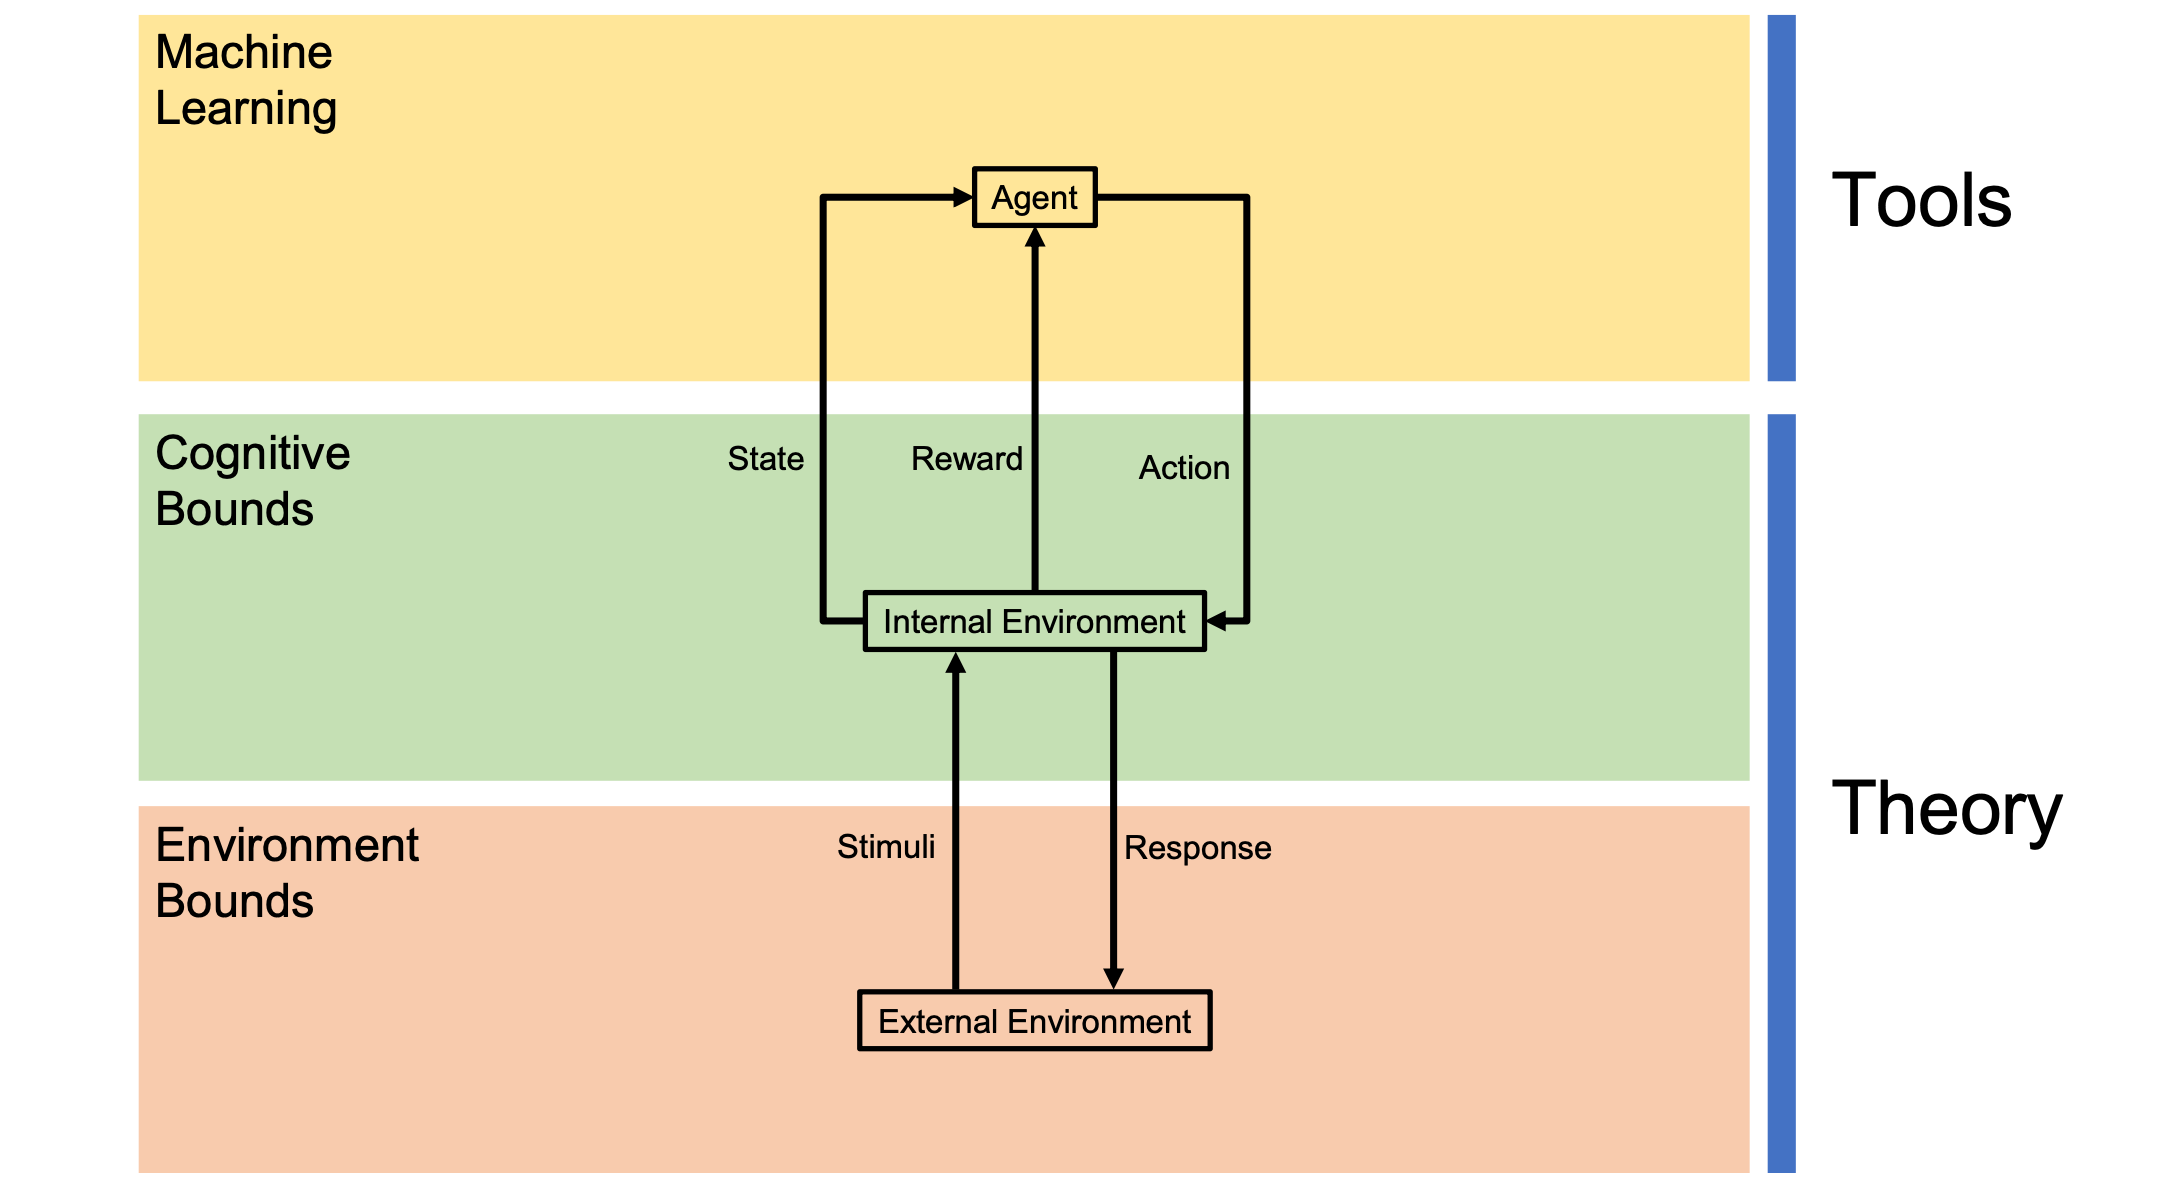
\includegraphics[width=\linewidth]{ml_and_bounds.png}
\end{center}




\begin{center}
	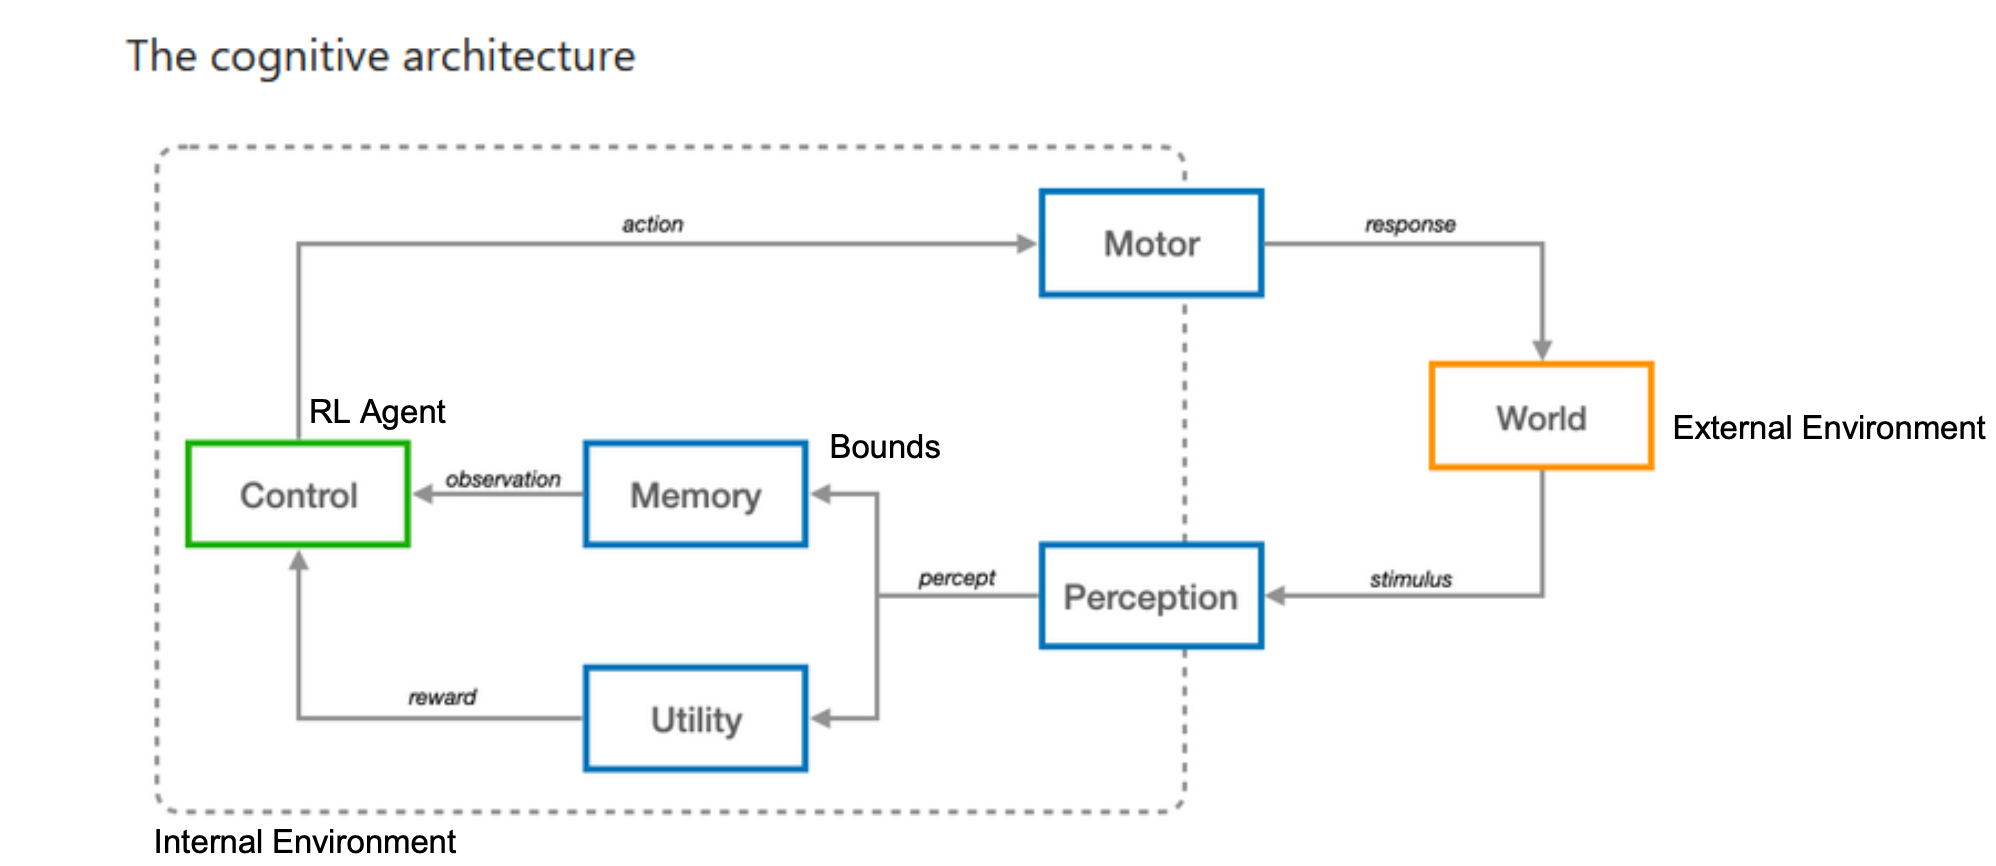
\includegraphics[width=\linewidth]{cognitive_architecture.png}
\end{center}


\textbf{Key cognitive capacities in HCI} \smallskip


\textit{General props of Human Cognition} \smallskip


\textit{1. Cognition is goal oriented} \smallskip


\textit{2. Cognition Adapts} \smallskip


\textit{3. Cognition Learns} \smallskip

\textit{4. Cognition computes based on internal representations} \smallskip

\textit{5. Cognition is limited \& costs energy} \smallskip

\textit{Perception} \smallskip


\textit{Elementary perceptual Tasks} \smallskip


\textbf{Gaze-based Interaction} \smallskip


\textit{Comparison with Cognitive Architectures}


\begin{center}
	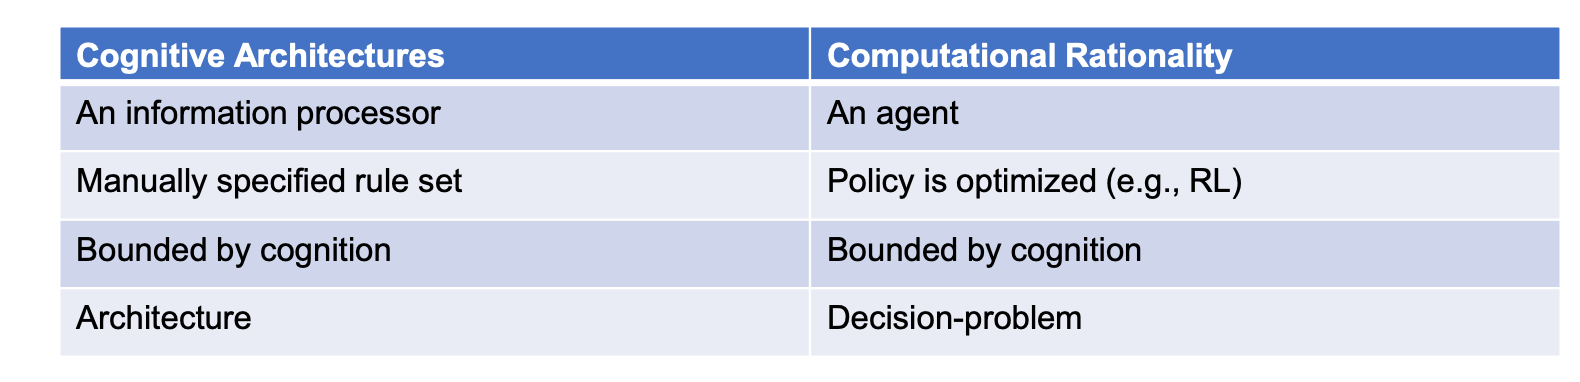
\includegraphics[width=\linewidth]{comparison_cognitive_architectures.png}
\end{center}












